% !TEX root = ../../../main.tex

\toggletrue{image}
\toggletrue{imagehover}
\chapterimage{dependency}
\chapterimagetitle{\uppercase{Dependency}}
\chapterimageurl{https://xkcd.com/2347/}
\chapterimagehover{Someday ImageMagick will finally break for good and we'll have a long period of scrambling as we try to reassemble civilization from the rubble.}


\chapter{Analyse der Turtle-Grundlagen}
\label{ch:analyse_der_turtle-grundlagen}

Bisher haben wir beim Programmieren stets von Befehlen gesprochen. In diesem Abschnitt geht es darum, etwas genauer hinzuschauen. Wir können Befehle in verschiedene Kategorien einteilen und werden uns nun mit den ersten Kategorien beschäftigen, die bisherigen Befehle analysieren und neue Fachbegriffe einführen. Die Ziele dieses Kapitels sind:\\

\lernziel{\autoref{ch:analyse_der_turtle-grundlagen}, \nameref{ch:analyse_der_turtle-grundlagen}}{
\begin{minipage}{\linewidth}
$\square$ \hspace{0.1cm} Sie erklären die neuen Fachbegriffe und geben dazu Beispiele.\\
$\square$ \hspace{0.1cm} Sie verknüpfen die Fachbegriffe mit einem gegebenen Python-Programm.\\
$\square$ \hspace{0.1cm} Sie recherchieren in der Python-Dokumentation.
\end{minipage}
}

\section{Befehle analysieren}
\label{sec:befehle-analysieren}

Wir besprechen die neuen Fachbegriffe anhand von \autoref{lst:quadrat-2}. Das Programm besteht aus zehn Befehlen, die wir in zwei Kategorien einteilen können:

\begin{itemize}
    \item \lstinline[language={python3}]{import}-Anweisung
    \item Funktionsaufruf
\end{itemize}

Woher weiss ich, zu welcher Kategorie ein Befehl gehört? Diese Information müssen Sie in der Beschreibung zur Programmiersprache nachlesen. Wir bezeichnen diese Beschreibung als \textbf{Dokumentation}. Die Dokumentation für Python können wir unter \url{https://docs.python.org/} finden. Wir fassen in diesen Unterlagen für ausgewählte Befehle die wichtigsten Informationen aus der Dokumentation zusammen.

\begin{lstlisting}[language={python3}, caption={Python-Programm für ein Quadrat.}, label={lst:quadrat-2}]
import turtle

turtle.forward(100)
turtle.left(90)
turtle.forward(100)
turtle.left(90)
turtle.forward(100)
turtle.left(90)
turtle.forward(100)
turtle.left(90)
turtle.done()

\end{lstlisting}


\section{\lstinline[language={python3}]{import}-Anweisung}
\label{sec:import-anweisung}

Der Befehl in der ersten Zeile aus \autoref{lst:quadrat-2} (\lstinline[language={python3}]{import turtle}) gehört zur Kategorie \say{\textbf{\lstinline[language={python3}]{import}-Anweisung}}. Dadurch erhalten wir Zugriff auf die bereits vorhandenen Befehle. Die vorhandenen Befehle werden in \textbf{Modulen} verpackt. Software-Entwickler können Module erstellen und diese zur Verfügung stellen. Jedes Modul hat einen \textbf{Namen}. Diesen Namen geben wir in der \lstinline[language={python3}]{import}-Anweisung an. Die \lstinline[language={python3}]{import}-Anweisung lautet somit im Allgemeinen:

\begin{center}
    \lstinline[language={python3}]{import modulname}
\end{center}

In unserem Programm müssen wir dann \lstinline[language={python3}]{modulname} durch den gewünschten Modulnamen ersetzen.

\begin{important}
    Bitte beachten Sie, dass zwischen \lstinline[language={python3}]{import} und dem Modulnamen zwingend ein Leerzeichen eingefügt werden muss.
\end{important}

Es liegt in der Verantwortung des Programmierers sicherzustellen, dass der Modulname existiert.

\begin{example}
    Unsere bisherigen Programme verwenden das Turtle-Modul. Mit \lstinline[language={python3}]{import turtle} erhalten wir die Befehle, um die Turtle zu bewegen. Es gibt noch andere Module, die wir verwenden werden. Wir können etwa mit \lstinline[language={python3}]{import random} Befehle verwenden, um zufällige Zahlen zu erzeugen, oder mit \lstinline[language={python3}]{import math} erhalten wir Zugriff auf Befehle für mathematische Berechnungen (zum Beispiel Quadratwurzel ermitteln).
\end{example}

\subsection{Was ist der Vorteil?} Häufig verwendete Programmierelemente müssen nicht selbst erstellt werden. Wir können auf bestehende Module zurückgreifen und reduzieren so den Programmieraufwand.


\section{Funktionsaufruf}
\label{sec:funktionsaufruf}

Die Befehle in den Zeilen drei bis zehn und der Befehl in Zeile zwölf in \autoref{lst:quadrat-2} gehören alle zur Kategorie \say{\textbf{Funktionsaufruf}}. Jeder dieser Befehle stellt einen Funktionsaufruf (engl. function call) dar. Wir können eine vorhandene Funktion ausführen, indem wir einen \textbf{Funktionsaufruf} verwenden. Ein Funktionsaufruf führt Code aus, der unter einem Namen zusammengefasst ist. Wir erkennen einen Funktionsaufruf wie folgt:

\begin{center}
    \lstinline[language={python3}]{funktionsname(argumente)}
\end{center}

Ein Argument ist z.B.\ eine Zahl. Manche Funktionen benötigen mehrere Argumente. Manche Funktionen brauchen gar kein Argument. Vorerst \say{bedienen} wir uns an bereits existierenden Funktionen. Später werden wir sehen, wie wir \textbf{selbst} Funktionen erstellen können (Funktionsdefinition).

\begin{figure}[htb]
    \centering
    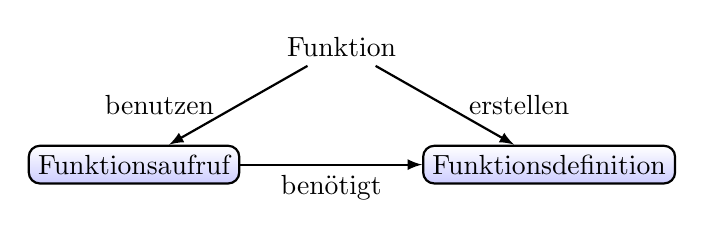
\begin{tikzpicture}[sibling distance=15em, edge from parent/.style = {draw, -latex, thick}]
        \node {Funktion}
        child { node[{shape=rectangle, thick, rounded corners,
        draw, align=center, top color=white, bottom color=blue!20}] (call) {Funktionsaufruf} edge from parent node [left, xshift=-0.5em] {benutzen}}
        child { node[{shape=rectangle, thick, rounded corners,
        draw, align=center, top color=white, bottom color=blue!20}] (def) {Funktionsdefinition} edge from parent node [right, xshift=0.5em] {erstellen}};
        \path[-latex, draw, thick] (call) edge node[below] {benötigt} (def);
    \end{tikzpicture}
\end{figure}

Betrachten wir nun einen bekannten Funktionsaufruf im Detail.

\begin{example}
    \label{example-function-call}

    Wir rufen die Funktion \lstinline[language={python3}]{forward} mit dem Argument \lstinline[language={python3}]{100} auf. Da die Funktion aus dem Turtle-Modul stammt, müssen wir den Modulnamen vor dem Funktionsaufruf notieren. Modulname und Funktionsaufruf werden durch einen \textbf{Punkt} miteinander verbunden.

    \[
        \begin{array}[t]{ccc}
            \underbrace{\textrm{\texttt{turtle}}}_{\textrm{Modulname}} & \underbrace{\textrm{\texttt{.}}}_{\textrm{Punkt}} &
            \begin{array}[t]{cccc}
                \underbrace{\textrm{\texttt{forward}}}_{\textrm{Funktionsname}} & \underbrace{\textrm{\texttt{(}}}_{\textrm{öffnende Klammer}} & \underbrace{\textrm{\texttt{100}}}_{\textrm{Argument (eine Zahl)}} & \underbrace{\textrm{\texttt{)}}}_{\textrm{schliessende Klammer}}
            \end{array} \\
            & & \underbrace{\hspace{11cm}}_{\textrm{Funktionsaufruf}}
        \end{array}
    \]

\end{example}

\subsection{Was können wir als Argument verwenden?}

Wenn ein Funktionsaufruf ein Argument benötigt, dann müssen wir in der Dokumentation nachschauen, was wir als Argument verwenden können. Ein Funktionsaufruf kann nicht mit jedem Argument verwendet werden. \textbf{Argument und Funktionsaufruf müssen zusammenpassen}. Für alle Argumente haben wir bisher immer einen konkreten \textbf{Wert} verwendet: eine Zahl oder einen Text. Wir verwenden dafür die folgenden Fachbegriffe:

\begin{definition}[Integer]
    Eine ganze Zahl, wie zum Beispiel \lstinline[language={python3}]{17}, ist ein Integer Value. Wir sagen dafür kurz: \lstinline[language={python3}]{17} ist ein \textbf{Integer}.
\end{definition}

\begin{definition}[String]
    Ein Text, wie zum Beispiel \lstinline[language={python3}]{"turtle"}, wird \textbf{String} genannt. In Python benötigen wir für einen String die \textbf{doppelten} Anführungszeichen.
\end{definition}

\begin{example}
    Der Funktionsaufruf \lstinline[language={python3}]{forward(100)} verwendet den Integer \lstinline[language={python3}]{100}. Beim Funktionsaufruf \lstinline[language={python3}]{shape("turtle")} wird der String \lstinline[language={python3}]{"turtle"} benutzt.
\end{example}

\cleancoderegel{\autoref{ch:analyse_der_turtle-grundlagen}, \nameref{ch:analyse_der_turtle-grundlagen}}{
\begin{cleancode}[Leerzeichen 1]
    Mehrere \textbf{Argumente} werden durch ein \textbf{Komma} getrennt. \textbf{Nach} einem Komma notieren wir ein \textbf{Leerzeichen}.
\end{cleancode}
}

\section{Kommentare}

Wir können einen Python-Code mit \textbf{Notizen} versehen, die für die Ausführung \textbf{keine Rolle} spielen. Diesen Vorgang nennen wir \textbf{Code kommentieren}.

\begin{definition}[Python-Kommentare]
Mit dem \lstinline[language={python3}]{#} Symbol (Hash-Symbol) startet in Python ein Kommentar. Python ignoriert bei der Ausführung alles nach dem \lstinline[language={python3}]{#}. Kommentare sind also für uns Menschen gedacht, die den Quellcode lesen.
\end{definition}

Kommentare können wir direkt nach einem Befehl in derselben Zeile oder in einer separaten Zeile notieren. Wir können Kommentare auch über mehrere Zeilen verteilen. Dazu müssen wir pro Zeile ein Hash-Symbol notieren.

\begin{example}
Wir können z.B. Kommentare verwenden, um eine Code-Analyse durchzuführen.
\begin{lstlisting}[language={python3}, caption={Code-Analyse mit Kommentaren (\graybgtexttt{bsp\_1.py}).}, label={lst:code-analyse}]
import turtle

turtle.forward(100)  # Funktionsname: forward, Argument: <@\color{commentcolor}{100}@> (Integer)
turtle.left(90)
turtle.forward(100)
turtle.left(90)
turtle.forward(100)
# Modulname: turtle
# Funktionsname: left, Argument: <@\color{commentcolor}{90}@> (Integer)
turtle.left(90)
turtle.forward(100)
turtle.left(90)
turtle.done()

\end{lstlisting}
\end{example}



